\part{Formulating the research question}
\frame{\partpage}

\begin{frame}{What makes a good research question?}
	\begin{itemize}
		\pause\item \textbf{Motivates} and \textbf{focuses} your research
		\pause\item Is \textbf{relevant} to the field
		\pause\item Has \textbf{originality} (doesn't have to be completely original, but shouldn't be ``solved'')
		\pause\item Is \textbf{manageable} in the context of your project
		\pause\item Is neither \textbf{too broad} nor \textbf{too narrow}
		\pause\item Leads to \textbf{testable hypotheses}
		\pause\item Requires \textbf{argumentation} and \textbf{analysis}, not mere \textbf{statistics}
		\pause\item Is \textbf{interesting} and addresses a \textbf{need}
	\end{itemize}
\end{frame}

\begin{frame}{Scope of research questions}
	\begin{itemize}
		\pause\item Too broad:
			\begin{itemize}
				\item Are videogames bad for children?
			\end{itemize}
		\pause\item Too narrow, not interesting:
			\begin{itemize}
				\item How many children in Cornwall play Overwatch?
			\end{itemize}
		\pause\item Better:
			\begin{itemize}
				\item What effect does regular videogame playing have on the academic attainment of
					children ages 11--14?
			\end{itemize}
	\end{itemize}
\end{frame}

\begin{frame}{Research questions vs hypotheses}
	\begin{itemize}
		\pause\item A research question invites \textbf{exploration}
		\pause\item A hypothesis makes a \textbf{testable claim}
		\pause\item Research question:
			\begin{itemize}
				\item What effect does regular videogame playing have on the academic attainment of
					children ages 11--14?
			\end{itemize}
		\pause\item Hypothesis:
			\begin{itemize}
				\item There is a positive correlation in children ages 11--14
					between hours spent playing Minecraft and grades in computing
			\end{itemize}
		\pause\item A good research question leads to several hypotheses
	\end{itemize}
\end{frame}

\begin{frame}{Choosing a research problem}
	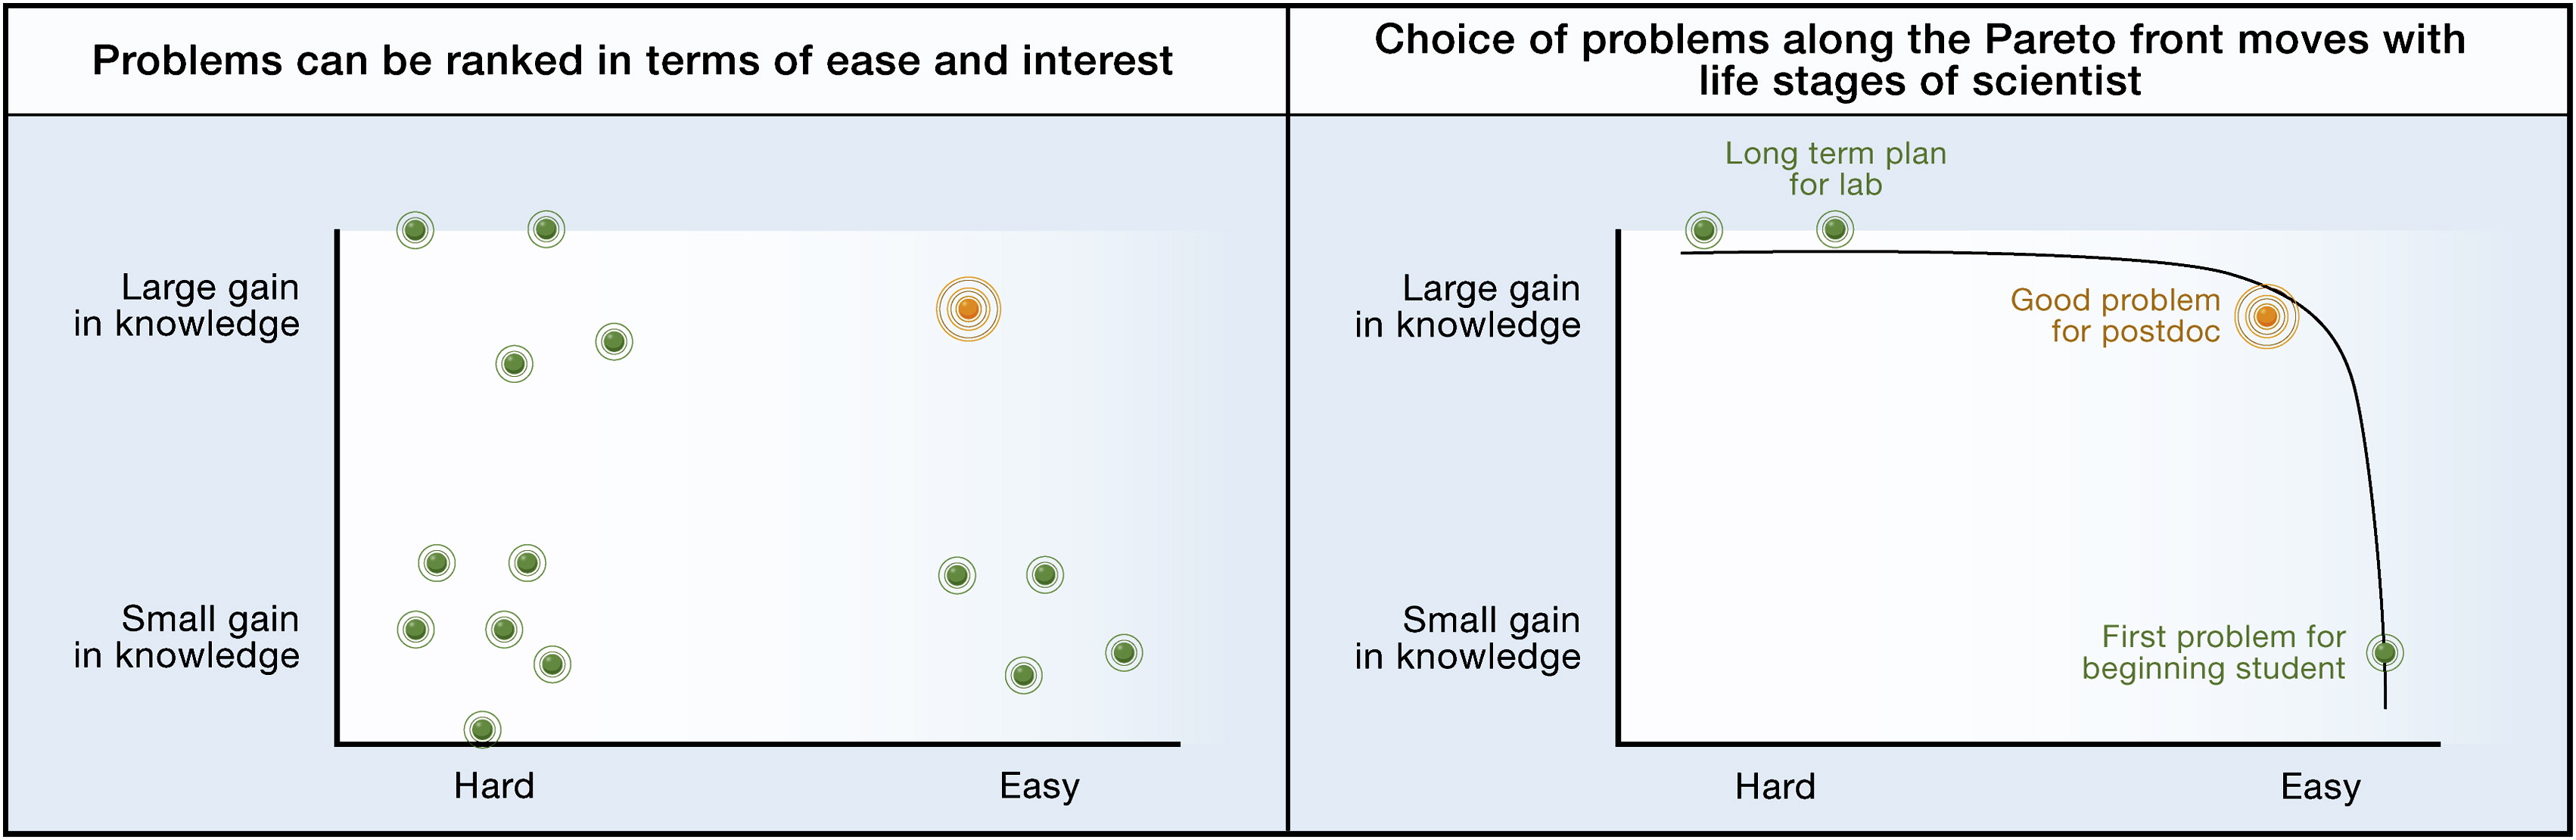
\includegraphics[width=\textwidth]{alon_fig1}
	
	{\tiny
	U.\ Alon, ``How to choose a good scientific problem,'' \textit{Molecular Cell} 35, pp.\ 726--728, 2009.
	}
\end{frame}

\begin{frame}{Exercise}
	\begin{itemize}
		\pause\item Look at some of the papers you have been reading
		\pause\item What are the \textbf{research questions} behind them?
	\end{itemize}
\end{frame}

